\chapter{Diffractive processes}
%\addcontentsline{toc}{chapter}{} 
\label{theoretics}

Diffractive dissociation has been studied for more than 50 years and therefore quite extensive theoretical theories have been created to achieve the goal of a successful description that corresponds with experimental results. The goal of this chapter is to introduce collisions, scatterings of particles and handy variables. Following will be a brief introduction to particle diffraction and in this part of particle physics, the quite successful Regge theory. At the end of the chapter, the process that is analyzed in \autoref{analysis} will be discussed, as well as the results from different experiments on the topic.

\section{Soft and hard processes}
Particle physics divides collisions into soft and hard collisions. Hard collisions are defined by two different energy scales of incident particles, often accompanied by relatively high momentum transfer\footnote{Momentum transfer is a quantity used in high energy physics. It is defined as the difference between the Lorentz vector of four-momentum of a particle before and after an interaction with another particle.} ($\geq$ $1$ GeV/c). Quantum chromodynamics (QCD), the theory of strong interactions, is very successful at describing hard collisions. On the other hand, typical for soft collisions are similar energy scales and, therefore, small momentum transfer. For soft interactions, QCD is not entirely accurate. Much more precise way to describe these processes is the Regge theory, which is more of a phenomenology\cite{Barone}. The goal for the last several decades has been to somehow incorporate, or be able to describe soft processes with QCD. Diffraction, as the main topic discussed in this thesis, belongs mainly to soft interactions. 
\section{Scattering}
Particle scatterings are distinguished based on their outcome. In this section, I will specify the interacting particles to be protons, but the same rules apply to all particle scatterings. Elastic and inelastic scattering. Elastic scattering is defined by the outcome,
\begin{equation}
\centering
p + p \longrightarrow p^{'} + p^{'}
\label{t1}
\end{equation}
when both incident particles are the same particles (without being excited) after the collision. Inelastic scattering (\autoref{t2}, \autoref{t3}) occurs when one or both of the incident particles are destroyed, creating a shower of partons that then hadronize. This is much more common for higher energy collisions. Elastic scatterings are much more easily measured.
\begin{equation}
\centering
p + p \longrightarrow p^{'} + X
\label{t2}
\end{equation}
\begin{equation}
\centering
p + p \longrightarrow X + Y
\label{t3}
\end{equation}
Particle physics separates collisions on one more condition: the properties of the detector. Some detectors are not capable of measuring all particles that take part in a collision. Such processes are called semi-inclusive or inclusive processes. Exclusive processes are, on the other hand, those when it is possible to measure all outcome particles, and therefore the physicist has all possible information about the product particles. In \autoref{analysis}, the focus will be on processes,
\begin{equation}
\centering
p + p \longrightarrow p^{'} + X + p^{'}
\label{t26}
\end{equation}
when 2 protons collide with transverse momentum being almost 0. Particle $X$ represents neutral particles, the scope of this thesis, which are reconstructed from hadron pairs. The processes then divide into 2 categories: resonance and continuum production. Resonance production happens when a neutral particle is created that then decays mostly to a hadron pair. Continuum production is the immediate creation of a hadron pair with total electric charge being 0. In either case, only the the decay pair is measured by the detector. More in \autoref{Pomeronprocess}. 



\section{Kinematic variables and quantities}
First, the simplest problem of 2 colliding particles is described. Because of the high energies and velocities of particles, every collision is characterized by the 4-momentum vector, which has to be conserved after the collision. Particle physics uses the Cartesian coordinate system, where $z$ is regarded as the direction of incident particles. Directions $x$ and $y$ are known together as the transverse plane. We are then able to introduce the Mandelstam invariants $s,$ $t$, and $u$, which are defined as,
\begin{equation}
\centering
s = (p_1 + p_2)^2 c^2 = (p_3 + p_4)^2 c^2
\label{t4}
\end{equation}
\begin{equation}
\centering
t = (p_1 - p_3)^2 c^2 = (p_2 - p_4)^2 c^2
\label{t5}
\end{equation}
\begin{equation}
\centering
u = (p_1 - p_4)^2 c^2 = (p_2 - p_3)^2 c^2
\label{t6}
\end{equation}
where $p_1$, $p_2$ are the 4-momentum vectors of incident particles and $p_3$, $p_4$ are 4-momentum vectors of outcome particles. Graphical representation of variables $s,~t,~u$ can be seen in \autoref{tf33}. As mentioned before, the 4-momentum vectors are Lorentz invariants in the Minkowski spacetime and, because of the conservation of energy and momentum, are equal for laboratory and center of mass coordinate systems. Variable $s$ denotes energy before and after the collision. Variable $t$ can be understood as particle 1 colliding with an antiparticle (particle with opposite direction of momentum and all additive quantum numbers with opposite sign) to particle 3. Variable $u$, which is not used very often, is analogous to $t$. Only the colliding particles are 1 and antiparticle to 4. Variables $s$, $t$ and $u$ satisfy the following equation.
\begin{equation}
\centering
s + t + u = \sum_{i=1}^4 m_i^2c^4
\label{t7}
\end{equation}
Variables $m_i$ are the respected masses of particles. This means that only 2 of the 3 variables are independent. Most of the time $s$ and $t$ are used. The different variables can also be understood as interactions through 3 different channels illustrated in \autoref{tf33}.
\FloatBarrier
\begin{figure}[ht]
    \centering
    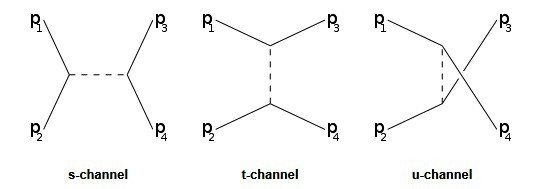
\includegraphics[width=1\textwidth]{figures/stu.jpg}
    \caption[Particle interactions through $s$, $t$, and $u$ channels]{Respective $s$, $t$ and $u$ channels for proton interactions.}
    \label{tf33}
\end{figure}
\FloatBarrier
Another two variables which are very important in particle physics are rapidity and pseudorapidity. Rapidity is defined as
\begin{equation}
\centering
y=\frac{1}{2}ln\left(\frac{E + p_zc}{E - p_zc}\right)
\label{t10}
\end{equation}
where $E$ stands for energy of a particle and $p_z$ momentum along the $z$ axis. Rapidity is also regarded as "velocity in the longitudinal direction" in high energy physics because  rapidity reduces to velocity in the non-relativistic limit. Rapidity is not a Lorentz invariant but it does hold a large role in detector physics. Pseudorapidity, $\eta$, is defined as the following,
\begin{equation}
\centering
\eta = -ln\left(tan~\frac{\theta}{2}\right)
\label{t11}
\end{equation}
where $\theta$ is the angle between the direction of an outcome particle and the $z$ axis. Pseudorapidity does have an advantage over rapidity- it is represented only by 1 independent variable, while rapidity needs energy and momentum to be defined. For high energy collisions, when it is possible to neglect the mass of particles, rapidity, and pseudorapidity coincide. Pseudorapidity ranges from 0 to infinity. Small angles of $\theta$ characterize diffraction therefore, the values for pseudorapidity of scattered protons are very big. 
\newline
The last and most important quantity of particle physics is cross-section $\frac{\mathrm{d}\sigma}{\mathrm{d} \Omega}$. The differential cross section is the probability per unit solid angle that an incident particle is scattered into the solid angle $\mathrm{d}\Omega$ \cite{Krane}. For easier computation, some assumptions have to be made. The densities of incident particles and target particles are considered to be small enough that they interact only once with each other, and that the energy that binds the target particles to their place is negligible compared to the energy of the incident particles. It is recognized as $\sigma$, but much more often, it is used in differential form as $\frac{\mathrm{d} \sigma}{\mathrm{d} x}$, where $x$ is a kinematic variable.
\begin{equation}
\centering
R_{int} = L \frac{\mathrm{d} \sigma}{\mathrm{d} \Omega}(\theta, \varphi)
\label{t25}
\end{equation}
\autoref{t25}, is a typical equation for the interaction rate $R_{int}$ of particles colliding in a collider. $L$ is luminosity, and it represents the properties of the collider, but not the particles themselves. Luminosity can be quite difficult to measure accurately. Therefore, it is one of the biggest sources of errors in collider physics. $\frac{\mathrm{d} \sigma}{\mathrm{d} \Omega}(\theta, \varphi)$ is the differential cross-section depending on the scattering angle. 

\FloatBarrier
\begin{figure}[ht]
    \centering
    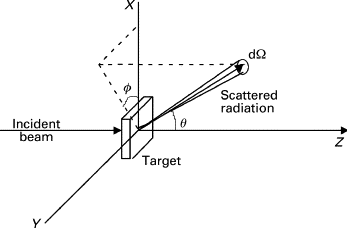
\includegraphics{figures/cs.png}
    \caption[Diagram of a scattering of a particle]{Diagram of a scattering of a particle into the solid angle $\mathrm{d}\Omega$. Taken from Ref.~\cite{cs}.}
    \label{tf32}
\end{figure}

\section{Particle diffraction}
The name diffraction comes from the analogy with optical diffraction, which is a phenomenon that occurs when a plane electromagnetic wave moves through a hole in a screen. The wave behind the screen lands on a detector plane, where intensity is measured. The Huygens-Fresnel principle states that every point in the hole in 
the screen becomes a unique source of a spherical electromagnetic wave, and what one can see on the detector is the interference of these sources of light. The analogy between particle and optic diffraction is the collision or interaction of 2 objects with similar wavelengths\footnote{Thanks to de Broglie hypothesis, it is possible to look at quantum particles as waves.}. The wave description is used because diffractive interaction is an ultra peripheral process. Particle diffraction has several definitions. The first definition was formulated by Good and Walker~\cite{GoodWalker} in 1960:
\newline
\newline
\textit{A reaction in which no quantum numbers are exchanged between the colliding particles is, at high energies, a diffractive reaction.}
\newline
\newline
In other words, diffraction has to satisfy 2 conditions- no quantum numbers\footnote{Quantum numbers understood as electrical charge, orbital angular momentum, spin, parity...} can be exchanged, and the collision must be at high energies. It is quite a straight-forward definition yet not entirely practical.  That is why an equivalent and more practical definition was formulated in lectures at Stanford University by Bjorken~\cite{Bjorken} in 1994.
\newline
\newline
\textit{A diffractive process occurs if and only if there is a large rapidity gap in the produced particle phase space, which is not exponentially suppressed.}
\newline
\newline
It translates to a simple condition that between forward and backward scattered protons and the hadron pair have to exist clear gaps in rapidity. Large rapidity gap is not exclusive for diffractive events, but all other events are exponentially suppressed. The number of diffractive events is somewhat constant with different energy of collision. In the next part, I will reproduce the calculation of the Large rapidity gap, as it is described in Ref.~\cite{Barone}. Even though it is almost an identical recreation, it is crucial for this thesis and the topic of diffraction. The computation and the following physical results are noted using natural units\footnote{Computation with natural units assumes the universal constants such as $\hbar$ or $c$ to be equal to 1.}.
\newline
Let us consider a high energy semi-inclusive collision where $p_1$, $p_2$ are 4-momentum vectors of colliding particles and $p_3$ represents the 4-momentum of an unaltered particle after the collision. For simplicity, the masses of the 3 particles are all the same and equal to $m$. 
\begin{equation}
\centering
p_1 = (E_1,0,0,p_z)
\label{t13}
\end{equation}
\begin{equation}
\centering
p_2 = (E_2,0,0,-p_z)
\label{t14}
\end{equation}
\begin{equation}
\centering
p_3 = (E_3,p_x^{'}, p^{'}_y ,p_z^{'})
\label{t15}
\end{equation}
As mentioned before, because of cylindrical symmetry, transverse momentum is used $p^{'}_T = \sqrt{p_x^{'2} + p_y^{'2}}$. Because the transverse momentum before the collision is 0, this condition has to be the same also after the collision, and therefore the sum $p_T$ of all product particles must equal to 0. In high energy approximation, the following equations are achieved,
\begin{equation}
\centering
\left|p^{'}\right| \approx \frac{s - M^2}{2\sqrt{s}}
\label{t17}
\end{equation}
\begin{equation}
\centering
\left|E_3\right| \approx \frac{s - M^2}{2\sqrt{s}}
\label{t18}
\end{equation}
where $M$ corresponds to the mass of a system of particles $X$, which is not measured. $s$ is above mentioned Mandelstam variable. Because a diffractive process is considered, transverse momentum will be significantly smaller than momentum along $z$ axis, therefore $\left|\vec{p}_z^{~'} \right| \simeq \left| \vec{p}^{~'} \right|$. It is possible to establish a variable called transverse mass,
\begin{equation}
\centering
m^{'}_{T} = \sqrt{m^2 + p^{'2}_{T}}
\label{t24}
\end{equation}
which is invariant under Lorentz transformation. Once again, if the mass of particles is approximated to be insignificant, the rapidity takes the form of the following equation.
\begin{equation}
\centering
y \approx ln \frac{2p_z}{m_{T}}
\label{t16}
\end{equation}
If all the aforementioned relations are combined, the rapidity of the 3. particle can be obtained.
\begin{equation}
\centering
y_3 \approx ln \frac{\sqrt{s}}{m^{'}_{T}}
\label{t19}
\end{equation}
The maximum value for this quantity corresponds to transverse momentum $p_{T}=0$.
\begin{equation}
\centering
y_{3max} \approx ln \frac{\sqrt{s}}{m}
\label{t20}
\end{equation}
The average and maximum value of the rapidity of system $X$ can be easily obtained.
\begin{equation}
\centering
\left<y_X\right> \approx -ln \frac{\sqrt{s}}{M}
\label{t21}
\end{equation}
\begin{equation}
\centering
\left|y_{X}\right|_{max} \approx ln \frac{\sqrt{s}}{m}
\label{t22}
\end{equation}
From these relations the rapidity gap between particle 3 and edge of the distribution of $X$ system takes the form of \autoref{t23}.
\begin{equation}
\centering
\Delta y \approx ln \frac{s}{M^2}
\label{t23}
\end{equation}
Because the mass of particles is neglected, pseudorapidity takes the same exact form.
\FloatBarrier
\begin{figure}[ht]
\centering
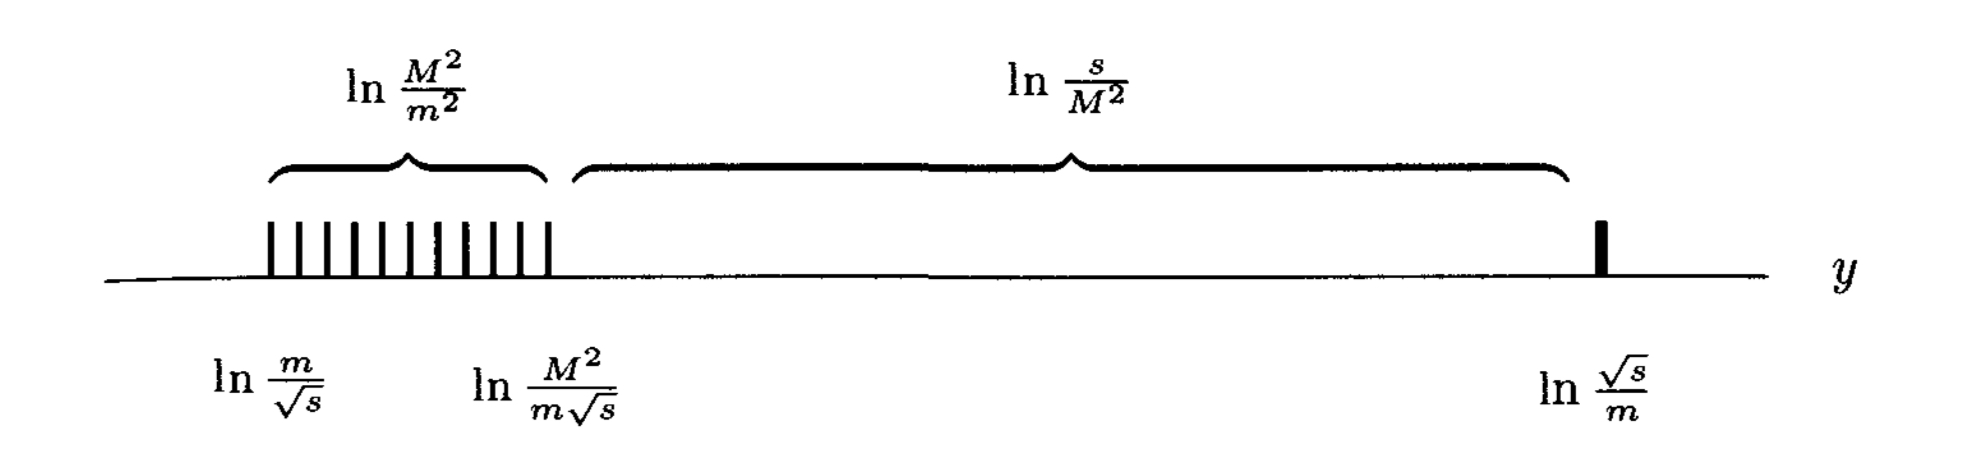
\includegraphics[width=1\textwidth]{figures/rapiditygap.jpg}
\label{tf1}
\caption[Large rapidity gap]{Graphical representation of rapidity gap between the unaltered particle 3, which is on the right side, and the system of particles $X$, which is on the left side. Taken from Ref.~\cite{Barone}.}
\end{figure}
\FloatBarrier


\section{Introduction to Regge theory}
One of the main ideas of Quantum mechanics is the fact that some variables are discrete. In other words, energy or angular momentum are not a continuous spectrum but can occupy only certain permitted values. These values depend later on the type of system and it's properties. Regge~\cite{Regge}, with his theory, went beyond that. He discusses the idea of extending the angular momentum range not only to all real values but also to complex values. Regge explained his idea on the scattering of a quantum particle on potential. He introduced complex angular momentum which depends on the energy of the collision. Such an approach leads to the distribution of energy which is known as Breit-Wigner energy distribution\footnote{Breit-Wigner distribution is a consequence of Heisenberg uncertainty principle. Incorporating a complex variable in quantified values results in the distribution of the quantity, and therefore, the uncertainty of the exact value. More in Ref.~\cite{Breit1936}}. Even though the theory is called after Tullio Regge, great contributions came from Geoffrey Chew and Steven Frautschi, who established a connection between Regge's extension of angular momenta and actual particles. Regge began the thought process by proposing that mesons and baryons are only bound states. Later Chew and Frautschi advanced the idea by stating that none of the bound states were elementary particles. They also followed up on Regge's trajectories idea by dividing known particles into several groups or families with similar quantum numbers which were based on their dependence of angular momentum on their squared masses. These families are represented in the so-called Chew Frautschi plot~\cite{ChewFrautschi} and can be seen in \autoref{tf4}.  
\newline
The full understanding of Regge theory is far beyond the scope of this thesis, but to introduce \Pom omeron physics it is necessary to understand what does reggeon\footnote{Reggeons are to be understood as something in Regge theory, that is exchanged between 2 particles that collide.} exchange mean. For the purpose of this thesis, high energy collisions with relatively low energy transfer will be considered an the spin of the scattered particle will be neglected. The partial wave expansion of the scattering amplitude $A(s,t)$ can be written as,
\begin{equation}
    \centering
    A(s,t)=16\pi \sum_{l=0}^{\infty}(2l + 1)A_l(s)P_l(cos~\theta_s)
    \label{t27}
\end{equation}
where $P_l(cos~\theta_s)$ is the Legendre polynomial of the appropriate wave amplitude. For fixed energy of collision, $s$, it is possible to reduce the dependence from energy transfer $t$ to only the scattering angle $\theta_s$. Consequently, it is possible to rewrite the dependence $A(s,t) \rightarrow A(s,t(s, cos~\theta_s))$. If equal mass of both incident particles is considered the following equation holds significance.
\begin{equation}
    \centering
    cos~\theta_s = 1 + \frac{2s}{t - 4m^2}
    \label{t28}
\end{equation}
In the limit of $s \rightarrow \infty$, the right-hand side grows quickly and Legendre polynomials are proportional to $s^l$. The partial wave amplitude then reduces to,
\begin{equation}
    \centering
    A_l(s,t) \sim f(t) s^{I}
    \label{t29}
\end{equation}
where $I$ is the spin of the exchanged particle for the certain partial amplitude. Optical theorem states $\sigma_{tot} \sim s^{I - 1}$, where $\sigma_{tot}$ is the total cross section. If all resonance exchanges are summed together and Regge's mathematical representation is used, it is possible to rewrite the partial wave amplitudes to be the following.
\begin{equation}
    \centering
    A(l,t) = A_l(t), {\color{white} \longrightarrow} l = 0, 1, 2...
    \label{t30}
\end{equation}
\begin{equation}
    \centering
    l=\alpha(t)
    \label{t31}
\end{equation}
Complex functions $\alpha(t)$ create poles in the complex $l$ plane. The sum of all the partial wave amplitudes gives the resulting scattering amplitude along with the total cross section shape~\cite{PomeronPhysics}. For \DPE~between 2 protons, the shape is shown in \autoref{tf5}. The total cross section is rising, which was first stated by Gribov and is well described in Ref.~\cite{gribov2003}.
\FloatBarrier
\begin{figure}[ht]
    \centering
    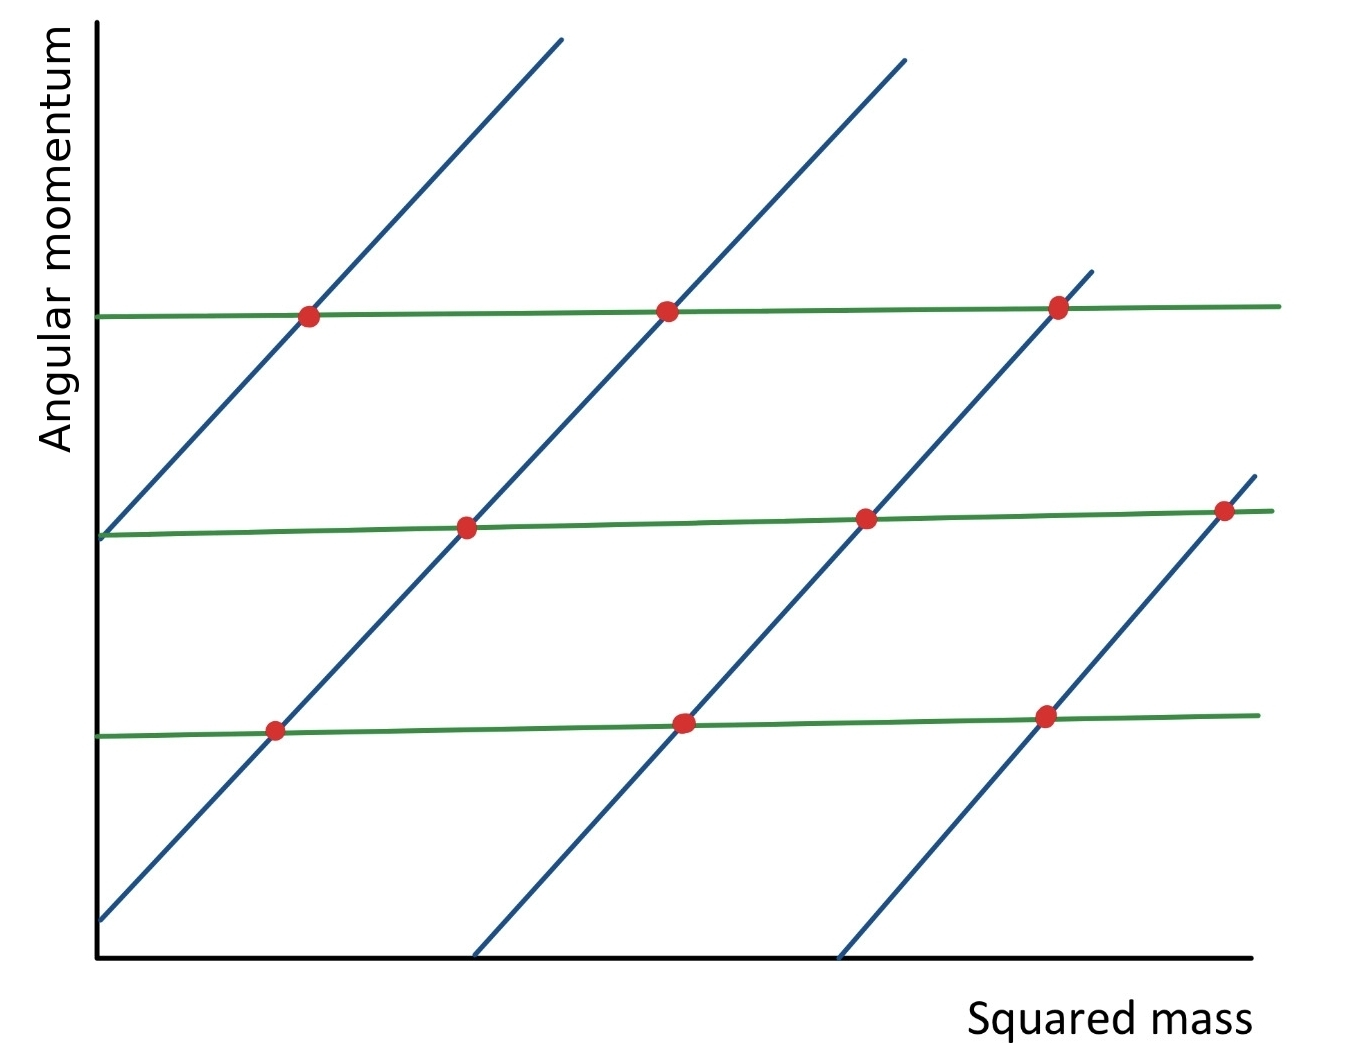
\includegraphics[width=0.7\textwidth]{figures/CFplot.jpg}
    \caption[Chew-Frautschi plot]{The Chew Frautschi plot of angular momentum dependence on squared mass. Blue lines represent Regge trajectories and red intercepts represent the bound states of particles. }
    \label{tf4}
\end{figure}
\FloatBarrier
\section{Pomeron process}
\label{Pomeronprocess}
\Pom omeron is a Regge trajectory, typical for diffractive events. It takes the name after the soviet physicist, Pomeranchuk, who has contributed to particle physics in many ways including the Pomeranchuk theorem which states that under some conditions the total cross sections of a particle and a corresponding antiparticle scattering on the same target becomes asymptotically same~\cite{PomeronPhysics}.
\newline
In this thesis, proton proton diffractive events at the center of mass energy $\sqrt{s} = 510$ GeV are studied, which are very well described with the so-called Double \Pom omeron exchange (\DPE). Another process, which creates a different system of particles, is called photoproduction and is described with the exchange of one \Pom omeron and one virtual photon. As mentioned before, the measured process is \autoref{t26}. The detector then detects hadron pairs which are mostly $\pi^+ \pi^-$, sometimes $K^+ K^-$ or $p \overline{p}$. Some processes may include a combination of these particles. On the other hand, particle $J/\psi$ decays to an electron-positron pair.
\FloatBarrier
\begin{figure}[ht]
    \centering
    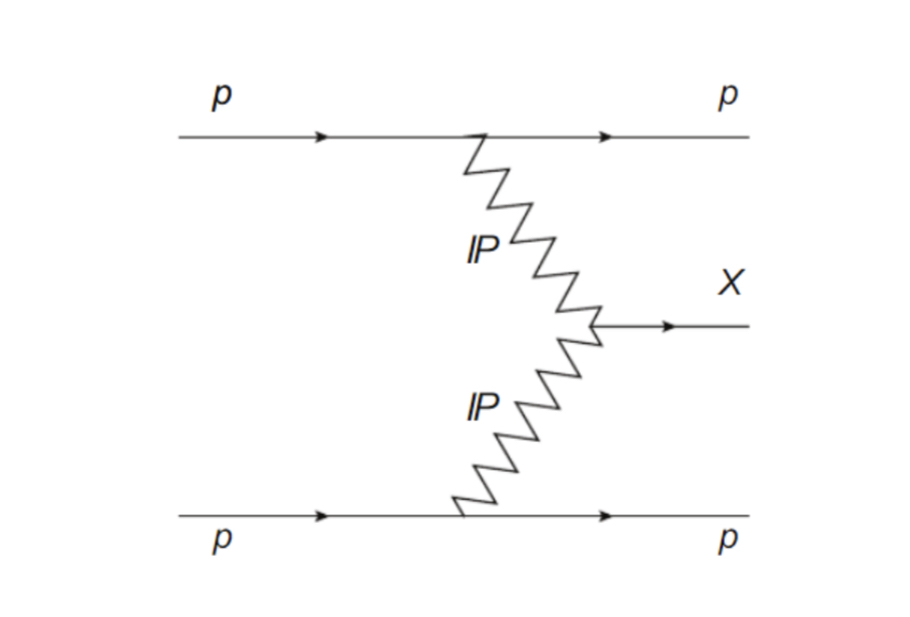
\includegraphics[width=0.7\textwidth]{figures/pomeronprocess.jpg}
    \caption[Double \Pom omeron exchange]{Double \Pom omeron  process between 2 protons with the result of the creation of another particle. The crisscross line represents the exchange of a \Pom omeron. Feynman diagram taken from Ref.~\cite{Guryn2016}.}
    \label{tf3}
\end{figure}
\FloatBarrier
Even though Regge theory has been developed for quite some time, the physical meaning of \Pom omeron is still quite unclear. The quantum numbers of \Pom omeron are the same as the quantum numbers of vacuum, isospin 0, and even charge parity, which does not correspond to any known particle. From experimental results, the \Pom omeron trajectory is expected to be a linear dependence on momentum transfer $t$~\cite{Albrow_2010}.
\begin{equation}
    \centering
    \alpha_{\mathbb{P}}(t) \sim \alpha_{\mathbb{P}}(0) + \alpha_{\mathbb{P}}^{'} = 1.08 + (0.25~\mathrm{GeV}^{-2})t
    \label{t32}
\end{equation}
Quantum chromodynamics describes the process (in the first approximation) as the exchange of 2 gluons. QCD predicts the existence of so-called glueballs, which are objects made up by 2 gluons or more. Glueballs have not yet been observed, but the studying the topic of \DPE~ will bring physicists closer to it's understanding and possibly even future confirmation, which would strongly support Quantum Chromodynamics. 

\section{Recent results}
\label{recent}
First of all, it is necessary to mention, that the measurement of $K^{0}_s$ (upon which will be the focus of this thesis) in diffractive proton-proton collisions at energies $\sqrt{s}=510$ GeV has never been done before. There have been similar measurements at experiment STAR and at different colliders and detectors. Even though there have been attempts to measure proton-proton collisions and \DPE~in the 1960s and 1970s, the first collider that was able to collide hadrons was the collider Intersecting Storage Rings (ISR). Previous experiments did not acquire enough energy to create 2 Large rapidity gaps~\cite{Albrow_2017}. Intersecting Storage Rings brought the first data of \DPE.
\FloatBarrier
\begin{figure}[ht]
    \centering
    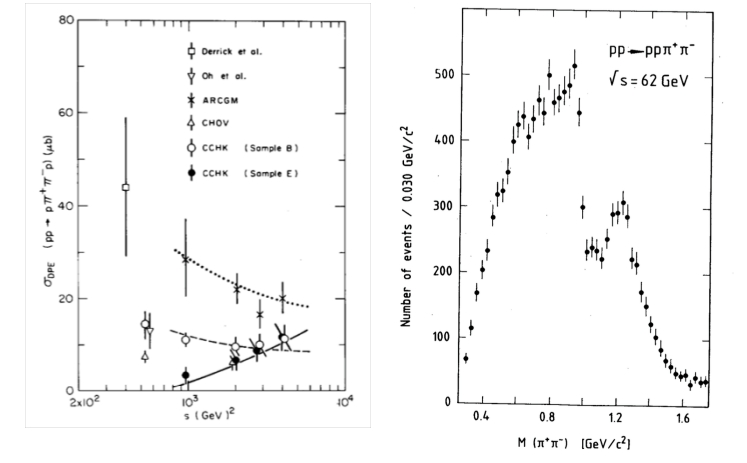
\includegraphics[width=0.9\textwidth]{figures/ISR.jpg}
    \caption[Cross section of pp collisions from ISR]{Left: Graph shows the dependence of cross section of \DPE~on ISR energies of collisions with respective fits of Regge trajectories. Right: Graph shows the central exclusive production of $\pi^{+}\pi^{-}$ production rate on invariant mass. Taken from Ref.~\cite{Albrow_2017}.}
    \label{tf6}
\end{figure}
\FloatBarrier
\FloatBarrier
\begin{figure}[ht]
    \centering
    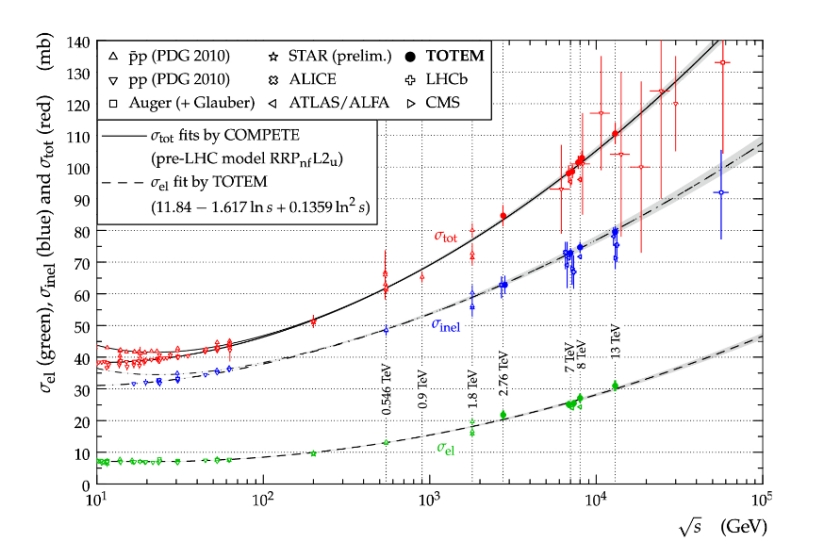
\includegraphics[width=0.9\textwidth]{figures/cspp.jpg}
    \caption[Cross section of pp and p$\overline{p}$ from different experiments]{Graph of cross section dependence on energy of proton-proton or proton-antiproton collisions measured at experiments STAR, ALICE, ATLAS, TOTEM, LHCb, CMS and AUGER. Green represents data from elastic collisions, blue is inelastic and red is total cross section. Taken from Ref.~\cite{zyla}.}
    \label{tf5}
\end{figure}
\FloatBarrier
The measurements of proton-proton collisions have gone a long way since the times of ISR. Such processes have been measured at all the significant experiments at different energies \autoref{tf5}. Most of the measurements are semi-exclusive: the outgoing protons are not tagged or measured. The only experiment, that is able to perform analysis on exclusive processes is the experiment STAR at RHIC, and it is thanks to subdetectors called Roman Pots. The latest article from the STAR collaboration on \DPE~is Ref.~\cite{Rafal20}, \textit{Measurement of the central exclusive production of charged particle pairs in proton-proton collisions at $\sqrt{s} = 200$ GeV with the STAR detector at RHIC}. The author discusses mainly the continuous creation of hadron pairs $\pi^+ \pi^-$, $K^+ K^-$, and $p\overline{p}$ and analyzes the cross section dependence on different variables such as the invariant mass of the created pair. 
\FloatBarrier
\begin{figure}[ht]
    \centering
    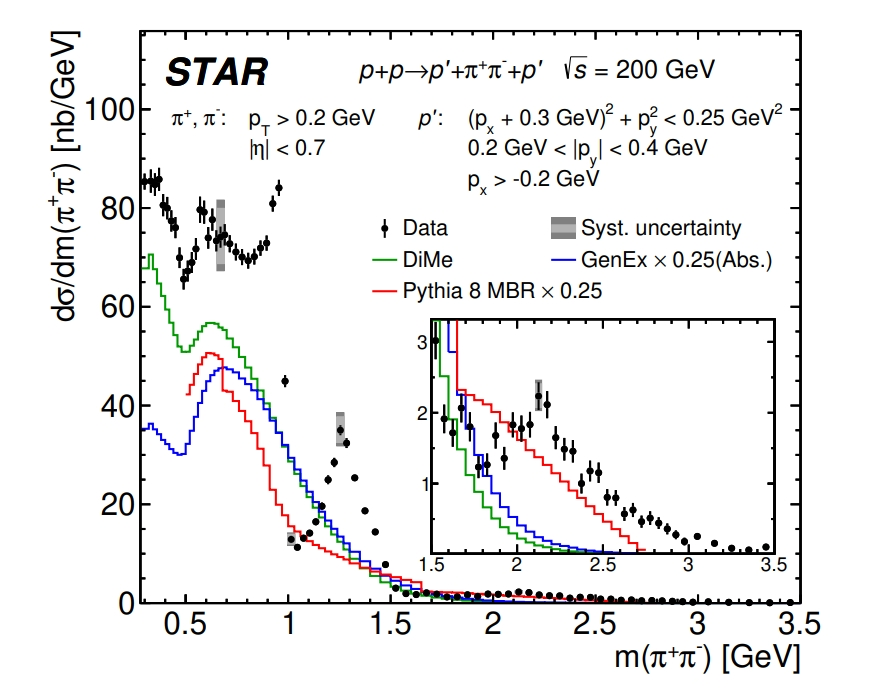
\includegraphics[width=1\textwidth]{figures/rafalpi.jpg}
    \caption[Cross section dependence on invariant mass for $\pi^+ \pi^-$ pairs at STAR]{Graph of cross section dependence on invariant mass of $\pi^+ \pi^-$ pair with 3 Monte Carlo simulations based on different phenomenological models. Taken from Ref.~\cite{Rafal20}.}
    \label{tf7}
\end{figure}
\FloatBarrier
For pion pair invariant mass, resonances $f_0$(980) and $f_2$(1270) were observed and expected to be the products of \Pom omeron- \Pom omeron fusion\footnote{\Pom omeron- \Pom omeron fusion is the continuous production equivalent to \DPE~in resonant production.}. Resonance $f_0$(980) can be seen in the graph at 0.98 GeV as a slight increase after which is a very steep drop. Resonance $f_2$(1270) follows after and can be seen at 1.27 GeV. Similar structures are seen in an independent study \cite{Truhlar}. 
\newline
According to Minkowski and Ochs, a very wide light scalar glueball might be located between 0.4 and 1.7 GeV. They call it the Red Dragon~\cite{Truhlar}. The same peaks can be seen in \autoref{tf6}. The author also noticed a resonance at around $\sim 2.2$ GeV which was not described by the Monte Carlo models. The simulations only predict continuous production and not the resonances.
\newline
Resonances $f_2$(1270) and $f^{'}_2$(1520) for kaons were measured, corresponding to previous measurements at lower energies. These resonances are also expected to be involving the \Pom omeron- \Pom omeron fusion. The statistics for $p\overline{p}$ were quite insignificant with large uncertainties, but there seems to be no significant resonances as in $\pi^+ \pi^-$ distribution.
\FloatBarrier
\begin{figure}[ht]
    \centering
    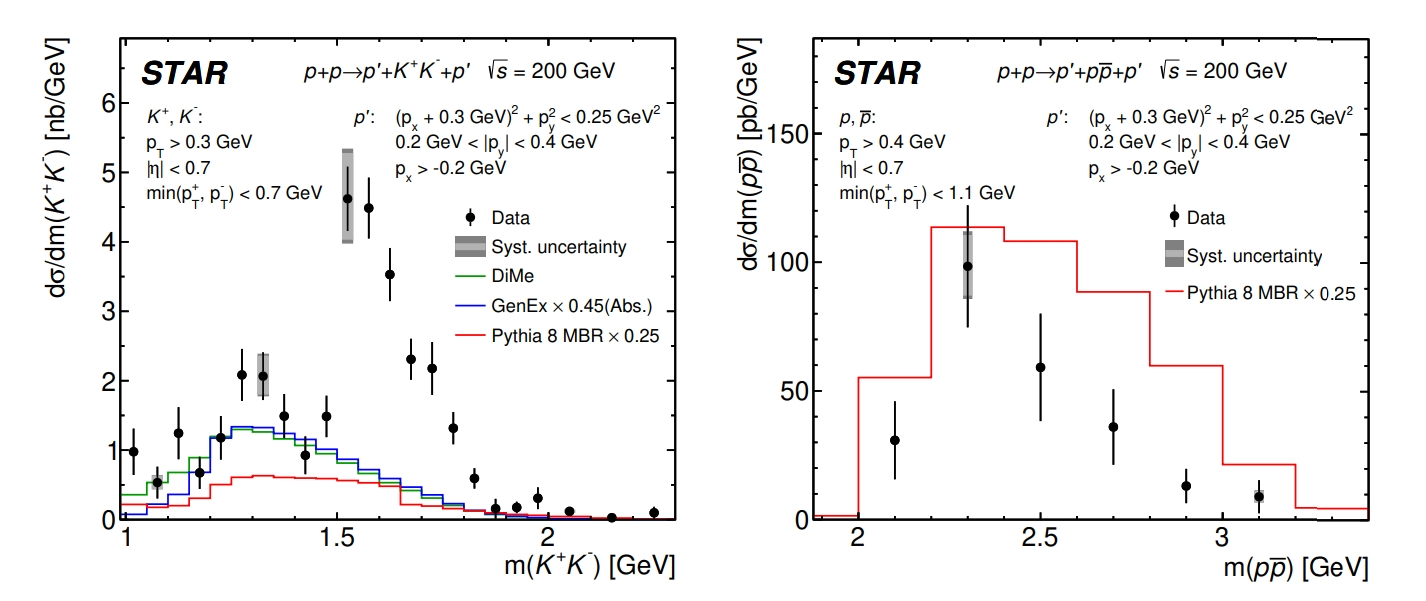
\includegraphics[width=1\textwidth]{figures/raphalkp.jpg}
    \caption[Graphs of cross section dependence on invariant mass of $K^+ K^-$ and $p \overline{p}$ pairs at STAR]{Graphs of cross sections dependence on invariant mass of $K^+K^-$ on the left and $p \overline{p}$ pairs on the right. Taken from Ref.~\cite{Rafal20}.}
    \label{tf8}
\end{figure}
\FloatBarrier
\begin{figure}[ht]
    \centering
    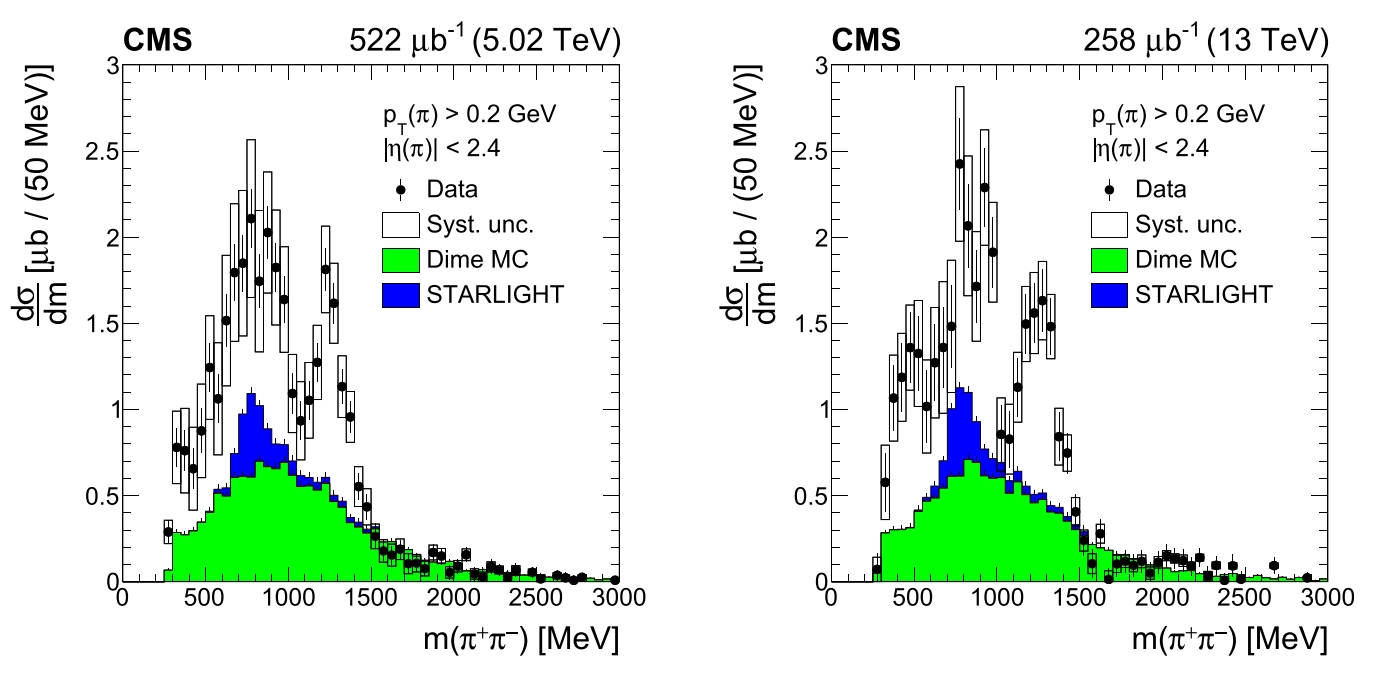
\includegraphics[width=1\textwidth]{figures/CMS.jpg}
    \caption[Cross section dependence on invariant mass of $\pi^+ \pi^-$ pairs at CMS]{Graphs of cross section dependence on invariant mass of created pion pair at $\sqrt{s}=5.02$ and $13$ TeV at CMS. Taken from Ref.~\cite{Sirunyan_2020}.}
    \label{tf8}
\end{figure}
\FloatBarrier
Another interesting measurement~\cite{Sirunyan_2020} was done at the CMS experiment at the Large hadron collider in CERN at energies $\sqrt{s} = 5.02$ and $13$ TeV. 4 resonant channels were extracted. The resonances are $f_0$(500), $\rho^0$(770), $f_0$(980) and $f_2$(1270). The latter 2 correspond previously mentioned resonances. Results for calculated cross sections of resonances are listed in table below.
\FloatBarrier
\begin{table}[ht]
    \centering
    \begin{tabular}{c|c|c}
        \
               & $\sqrt{s}$=5.02 TeV & $\sqrt{s}$=13 TeV \\ \hline
    $f_0$(500) & 2.8 $\pm$ 1.4(stat) $\pm$ 2.2(sys) & 2.2 $\pm$ 0.8(stat) $\pm$ 1.3(sys) \\
    $\rho^0$(770) & 4.7 $\pm$ 0.9(stat) $\pm$ 1.3(sys) & 4.3 $\pm$ 1.3(stat) $\pm$ 1.5(sys) \\
    $f_0$(980) & 0.5 $\pm$ 0.1(stat) $\pm$ 0.1(sys) & 1.1 $\pm$ 0.4(stat) $\pm$ 0.3(sys) \\
    $f_2$(1270) & 3.6 $\pm$ 0.6(stat) $\pm$ 0.7(sys) & 4.2 $\pm$ 0.9(stat) $\pm$ 0.8(sys) 
    \end{tabular}
    \caption[Results of measured cross sections for 4 resonant channels at CMS]{Table of total cross sections of observed resonances in pion production based on the energy of collisions. Data taken from experiment CMS~\cite{Sirunyan_2020}.}
    \label{tt1}
\end{table}
\FloatBarrier
